
% \begin{itemize}
%     \item Problem statement
%     \item Opportunity of voltage imaging, core idea of inverting the causal `presynaptic spike → postsynaptic PSP' relation
%     \item Overview of thesis
% \end{itemize}

% \section{Connectomics}

% \begin{itemize}
%     \item Motivation
%     \item Ground-truth connectomics: tracing of electron microscopy and fluoresent injection imaging
%     \item Necessity of connection \emph{inference}
%     \item Mention `invasive' connection testing (stimulate one cell, record possible neighbours)
%     \item Limitations of `connectomics', and of inferred vs `actual' connectomics.\\
%         Terminology, e.g. `functional connectomics'
% \end{itemize}


% \section{Voltage imaging}

% \begin{itemize}
%     \item Technologies (from dyes to GEVIs)
%     \item Specs: cell yield, tissue depth, recording duration, SNR, species
%     \item ..and growth of these over time, and comparison with calcium imaging.\\
%         To extrapolate how these might advance in the future
%     \item Comparison with other recording techniques: ephys, calcium imaging, (and briefly mention coarser methods)
% \end{itemize}


% \section{Network inference}

% \begin{itemize}
%     \item Working with events/spikes only, versus working with continuous signals; or a hybrid as here.
%     \item Overview of the spikes-only methods
%     \item The connectomics competition, and the findings about the best methods
%     \item Mention other application domains, like gene regulatory networks
%     \item Conclusion: connection inference by spikes is poor (Ila Fiete etc), and Vm imaging offers unique advantage (causality)
%     % \item 'Spike-triggered voltage regression' of Zhou/Cai
% \end{itemize}



The first section here gives an overview of the idea of this thesis, and its background. The second section delves a bit deeper into voltage imaging technology.



\section{Overview}

Systems neuroscience studies the links between (1) an animal’s behaviour, (2) the activity of its neurons, and (3) how these neurons are connected. Currently, only the first two can be observed simultaneously, using \emph{in vivo} recordings of neural activity. Observing the connections between neurons, on the other hand, requires imaging brain slices, and thus killing the animal. In addition, such a wire-tracing process is costly and time-consuming.

In this thesis, we aim to develop algorithms that infer the connections between neurons based on recordings of their voltages, instead of post-mortem imaging. We believe this is possible because the activity of neurons is mainly determined by the connections between them, and because recent advances in recording technology are yielding, for the first time, the necessary quality of data to solve this problem.

Such an algorithm then allows for fast and cheap estimation of the neural wiring in behaving animals, throughout their lifetime and across experiments. This could allow systems neuroscientists – whether they study e.g. memory, addiction, or movement disorders – to find answers to their questions linking brain wiring and brain (dys)function in a manner more straightforward than before.


\subsection{Recording neural activity}

There are currently two methods in popular use to record the activity of multiple individual neurons, in vivo: calcium imaging and extracellular electrode recordings. The strength of each method is the weakness of the other. Both are performed through a small, surgically created hole in the skull.

In calcium imaging, neurons are filled with a calcium indicator or “dye” – a molecule that becomes fluorescent when calcium binds to it. When a neuron sends an action potential (a “spike”), its cell body is briefly flooded with calcium. A dyed neuron that has just sent a spike thus becomes fluorescent for a short while. To record activity, laser light is focused in a point and scanned across a volume of brain tissue. Neurons that recently spiked will send light back, which is captured to yield a three-dimensional movie of neural activity. This allows scientists to observe large numbers of neurons – namely all active neurons in the volume. An additional advantage is that calcium indicators can be genetically targeted so that they only occur in specific neuron types of interest, providing a focused view. A major disadvantage however is that multiple spikes fired from a neuron in rapid succession cannot be easily distinguished, as the calcium effects of each spike are slow and combine non-linearly.

Extracellular electrode recordings on the other hand have a much finer time resolution and every spike is individually distinguishable. They work by inserting long, thin implants in the brain, that have many electrodes exposed on their surface. Each electrode measures the local electric field potential, and thereby picks up the spikes from nearby neurons. The increased time resolution comes at the cost of only sampling a small subset of the neurons in the areas of interest, not knowing exactly where those neurons are, and not being able to target neural subtypes specifically.

Calcium imaging thus provides good spatial information but has a low temporal resolution, whereas extracellular electrode recordings present the opposite trade-off: precise spike counts and timings, but limited spatial information and sampling of neurons. Recently, a recording technique is emerging that combines the advantages of both.


\FloatBarrier
\subsection{Voltage imaging}

\begin{figure}
    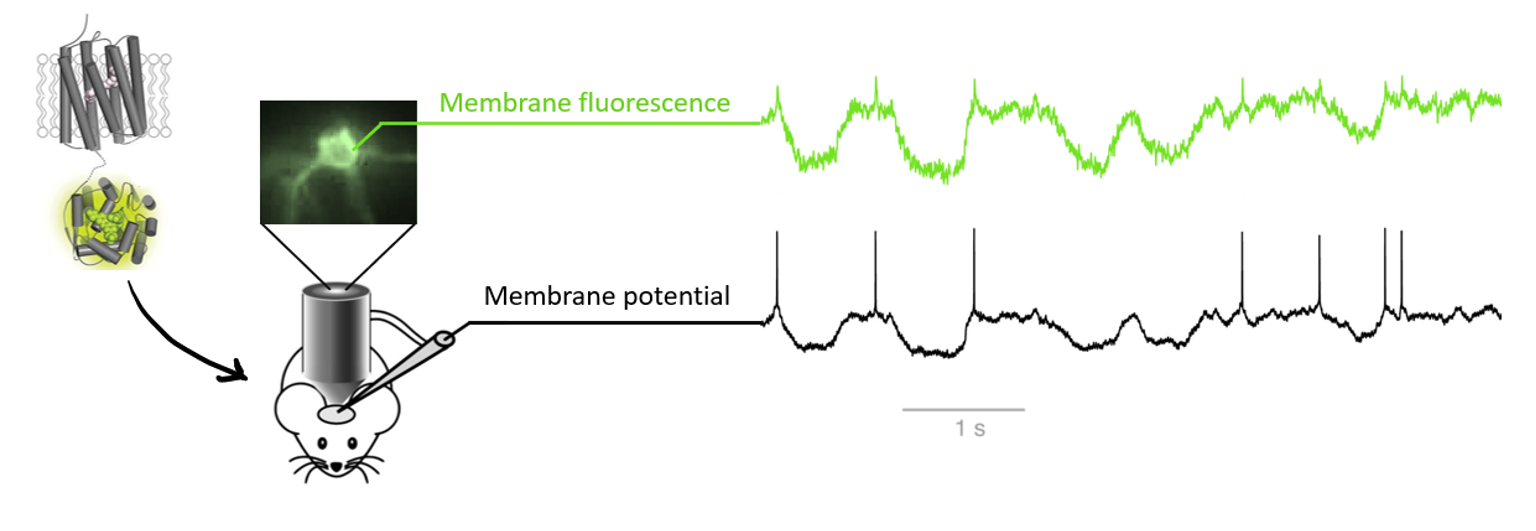
\includegraphics[w=1.5]{VI-sigs}
    \captionn{Voltage imaging}{
        Left: schematic of an example voltage indicator molecule embedded in the cell membrane. Middle: the imaging setup and an example neuron image. Right: an example voltage imaging trace and a simultaneous intracellular electrode recording.\\
        Adapted from \cite{Villette2019UltrafastTwoPhotonImaging,Abdelfattah2019BrightPhotostableChemigenetic}.
    }
    \label{fig:VI-sigs}
\end{figure}

Voltage imaging is very similar to calcium imaging: all or a genetically selected subset of neurons are made fluorescent, and these are scanned with a focused laser, to yield three-dimensional movies of neural activity. The difference is that the indicator molecules used in voltage imaging fluoresce in direct proportion to the membrane potential of the cell, instead of its calcium concentration. This then allows to directly observe the membrane potential of all neurons of interest in the field of view (\cref{fig:VI-sigs}).

Although voltage imaging has existed for a long time, the recorded signal has long been too weak to distinguish it from background noise (unless animals with very large neurons are used, or the activity of many co-firing neurons is pooled together). In recent years however, multiple labs have been iteratively refining the voltage indicator molecules. Together with the improvements in fluorescence imaging technology, driven by calcium imaging, this has made voltage imaging now powerful enough to image multiple individual neurons in vivo in common model animals. The signal-to-noise ratio has improved to the point that not only individual spikes, but also subthreshold voltage fluctuations can be observed.\footnote{
    \Cref{sec:voltage-imaging} further down expands further on the current capabilities of voltage imaging technology.
}
As explained next, it is precisely this level of detail that we believe enables in vivo connection mapping.


\subsection{Inferring wiring from activity}

\begin{figure}
    \vspace*{2em}  % space from vi fig above
    \hspace*{-2.5em}
    \includegraphics[w=1.2]{diagram_Connectivity↔Activity.png}
    \captionn
        {The causal link between neural connectivity and activity}
        {On the left, a cartoon of a synaptic connection. The axon of presynaptic neuron $M$ (in blue) impinges on postsynaptic neuron $N$ (in brown). The electrode icons indicate that their membrane voltages are recorded (shown on the right).
        A succesful spike in neuron $M$ will elicit a small but precisely-timed voltage bump in neuron $N$ (the postsynaptic potential, PSP).
        There is thus a causal relationship between 1) the existence of a connection $M$~→~$N$ and 2) both neurons' membrane voltages. This causal relationship (black arrow) is exploited to perform network inference from voltage recordings (green arrow).\newline
        \small{\emph{Drawings adapted from Purves et al.'s ``Neuroscience'' textbook, 6th edition, 2018.}}}
    \label{fig:diagram_Connectivity-Activity}
\end{figure}

The potential to infer the wiring from neural activity rests on the basic link between the two (\cref{fig:diagram_Connectivity-Activity}): an excitatory neuron that sends a spike will slightly increase the voltage of all its downstream neurons (this small increase is called the excitatory postsynaptic potential, or EPSP). When a neuron has received enough spikes, its voltage crosses a threshold, and it will send a spike itself. To estimate neural wiring, the idea is then to invert this reasoning: if neuron B often shows activity right after neuron A has fired, then neuron A is likely to be connected to neuron B.

As both calcium imaging and extracellular electrode recordings yield (at best) spike timing data only, existing activity-to-wiring approaches have been based only on spike timing, and not on more detailed measurements of neural activity. The problem with this is that the correlation between two neurons being connected and them spiking together close in time is quite tenuous. For one, most neurons need to receive many spikes – each of which can come from any of its hundreds to tens of thousands of input neurons – before it fires a spike itself. Second, many neurons have long time constants, meaning that a spike can influence spiking in its receiving neurons up to hundreds of milliseconds later.

As a result, spike-based wiring inference methods require very long recording durations to obtain some confidence on the wiring between even small numbers of neurons. During these long recordings, the connectivity may have already changed. And long recordings are not possible for fluorescence imaging, as dyes require recovery after each recording session.

When we can observe the subthreshold increases in voltage occurring directly after each spike however, we might be able to accurately reconstruct connectivity from recordings on the timescale of individual in vivo experiments. The recent advances in voltage imaging provide exactly this kind of data.



\clearpage
\section{Voltage imaging}
\label{sec:voltage-imaging}

What follows is a short literature review of the current capabilities of voltage imaging technology. The main goal is to be able to build simulations in this thesis relevant to reality.

\FloatBarrier

\begin{figure}
    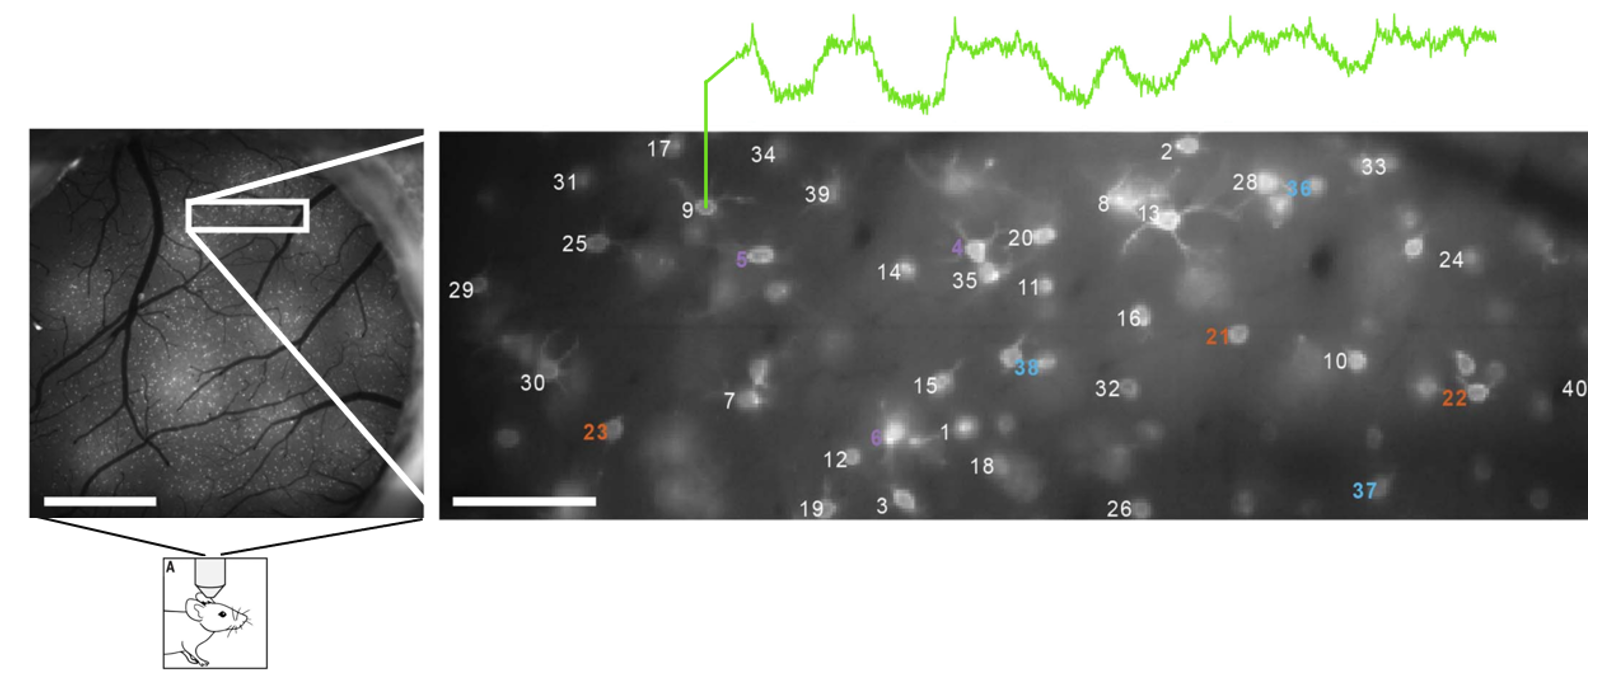
\includegraphics[w=1.5]{VI-cranial-window}
    \captionn
        {Camera view in voltage imaging}
        {Fluorescent neurons visible through a cranial window. This is just one imaging plane (i.e. there are more neurons visible above and below this plane). Voltage imaging recordings are thus 3D videos of neural membrane voltages.\\
        Adapted from \cite{Abdelfattah2019BrightPhotostableChemigenetic,Knopfel2019OpticalVoltageImaging}.}
    \label{fig:VI-cranial-window}
\end{figure}

\begin{figure}
    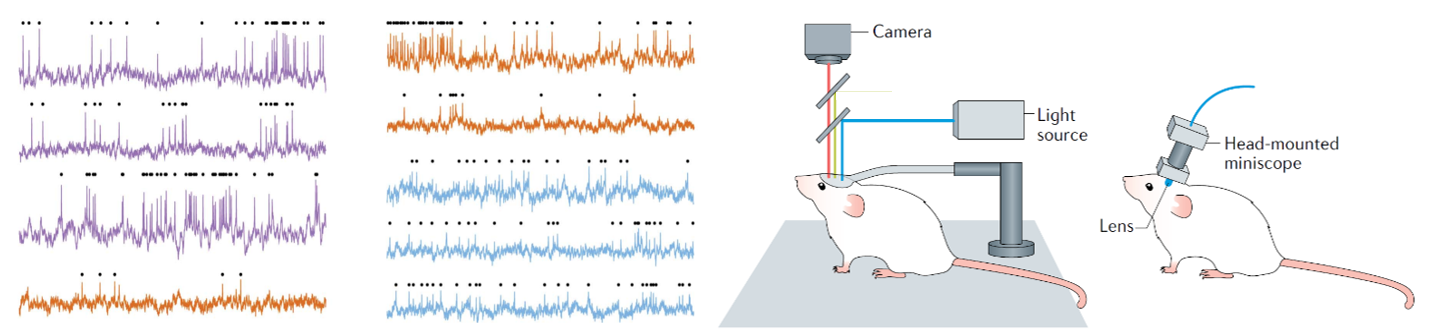
\includegraphics[w=1.5]{VI-sigs-and-setups}
    \caption
        {Left: More example VI traces, with different spike-signal-to-noise ratios. Colours correspond to neurons with coloured numbers in \cref{fig:VI-cranial-window}. Right: in-vivo imaging setups.\\
        Adapted from \cite{Abdelfattah2019BrightPhotostableChemigenetic,Knopfel2019OpticalVoltageImaging}.}
    \label{fig:VI-sigs-and-setups}
\end{figure}



\subsection{Working principle}

\subsubsection{Overview}

Voltage imaging is a type of fluorescence microscopy, itself a type of light microscopy. A light source such as a laser or an LED shines on the imaged object -- such as a slice of brain tissue, a young transparent zebrafish, or part of a mouse brain made accessible through a hole in the skull. Most light passes through the sample of interest (brain tissue is mostly transparent for the used wavelengths). However, some parts of the sample 'reflect' light back.

These reflecting parts are so called voltage indicator molecules. Such molecules are introduced by the experimenter and gather spontaneously in cell membranes. The amount by which they reflect light back depends on the voltage placed over them. By capturing the reflected light from a sample, repeatedly over time, we thus get a movie showing 1) where cell membranes are, and 2) how the voltages over them change over time.

\subsubsection{In more physical detail}
The above is a simplified description of the mechanics. This section gives a slightly more detailed description of what happens.

The actual mechanism of light 'reflection' is fluorescence, in which molecules absorb a photon, hold on to it for about one nanosecond, and then re-emit it again, at a longer wavelength. This process is about a million times slower than 'true' reflection (that is, photon scattering), but still a million times faster than the timescales we are interested in (milliseconds, corresponding to the duration of an action potential) and at which we image (with movie frame rates of 500 - 1500 Hz).

Furthermore, a change in voltage does not necessarily lessen the total fluorescence. Rather, the emission spectrum may shift. If you however only look at a fixed narrow band of the emitted light (as is done in fluorescence microscopy), the measured light will indeed seem to decrease or increase on voltage changes.
'Instantaneous reflection modulated by voltage' is thus a sufficient mental model for our purpose.

\subsubsection{Genetic targeting}

Since the late 90's, cells have been coerced into creating (parts of) indicator molecules themselves, by delivering transgenes into the cell. This has multiple advantages. Most importantly, it allows the indicator molecules to be constrained to only certain cell types, by placing the transgene under the control of promotors that are only active in the cell type of interest. By doing so, scientists can avoid labelling glial cells. This decreases the background signal. Going further with the same principle, they can selectively label one type of neuron (for example, only interneurons in one hippocampal area).

Another advantage, also decreasing the background signal, is that indicator molecules can be constrained to the membrane of only the cell body, and not the membranes of dendrites and axon branches. This is done by adding small cell-body-targeting signalling sequences to the transgene.



\subsection{System performance}

The history of voltage imaging has mostly been the history of finding better indicator molecules. Earlier versions (starting from their invention in the late 60's) changed their reflectance only weakly and slowly in response to a change in voltage. In addition, they were toxic, disrupting the normal functioning of cells, or altogether destroying them.
Modern indicators are no longer toxic, and their voltage sensitivity and speed have improved substantially (by more than ten- and hundredfold, respectively).


\subsubsection{Fidelity}

Current voltage indicators can have sub-millisecond time constants, meaning they can replicate the shape of an action potential as well as an electrode recording. During an action potential in a brain slice, the measured fluorescence of current voltage indicators increases by 30\% (± about 20\%)\footnote{
    Round brackets in this section indicate a rough indication of variation between experimental setups.
    See [this table (todo)] for concrete data from some representative VI studies.
    [data from \hyperlink{https://docs.google.com/spreadsheets/d/1W9Y3az4i1xdvahpdyqtsTG8F81LXK2T6wzRgsXHN3z0/edit}{this spreadsheet}].)
}
relative to baseline. In live, head-fixed mice, this fluorescence increase is about 8\% (± 2\%).

More important is the change in brightness with respect to noise. For voltage imaging, a signal-to-noise ratio (SNR) is often defined as the height of the fluorescence signal during an action potential, divided by the standard deviation of the baseline fluorescence signal.  The action-potential-SNR is around 30 (± 7) in brain slices, and around 10 (± 3) in live, head-fixed mice.

There has been no quantification yet of how well voltage indicators track subthreshold voltages. Estimating visually from published figures however, the correspondence between simultaneous electrode and optical recordings is substantial, and seems good enough to calculate with, even in recordings from live animals.


\subsubsection{Yield}

The number of simultaneously voltage-imaged neurons in live mice varies between 4 and 46 in the latest studies (with frame rates of mostly 500 Hz).

For comparison, calcium imaging yields between 200 and 1000 neurons at a frame rate of 30 Hz, and up to 10,000 at 2 Hz. These higher yields come of course at the cost of less information per neuron: voltage imaging tracks subthreshold voltages and detects nearly all spikes, while calcium imaging, especially at such frame rates, yields only spike detections, imprecise both in time and in number.

The number of simultaneously imaged neurons is in any case bound to increase for both modalities, as microscopic scanning systems get faster.

Voltage imaging can only be performed in relatively short continuous bouts: the same mechanism that makes the molecules fluorescent -- namely, excitation on impact of a photon -- also makes the molecules more chemically reactive, making them spontaneously break down ('photobleach') in reaction with their environment. The total fraction of not-yet photobleached indicator molecules decays exponentially -- and so do the fluorescence and the spike SNR. The time constant of this decay (i.e. duration after which SNR has decreased by 63\%) is around 10 ± 5 minutes. Most voltage imaging sessions are therefore not longer than this.

Cells replace broken indicator molecules relatively fast however, and experiments have shown that imaged photobleached cells show complete recovery after two days. Even shorter intervals between imaging sessions might be possible.

Because modern indicator molecules are not toxic, cells can be intermittently imaged over long periods -- one study followed the same neurons in vivo over more than a month.
